\documentclass[upright, contnum]{umemoria}

\depto{DEPARTAMENTO DE CIENCIAS DE LA COMPUTACI\'ON}
\author{NICOL\'AS MART\'IN MIRANDA CASTILLO}
\title{REGLAS DE ASOCIACI\'ON PARA L\'INEAS ESPECTRALES}
\auspicio{el D\'ECIMO NOVENO 
CONCURSO DE PROYECTOS DE INVESTIGACI\'ON Y DESARROLLO FONDEF 2011, 
PROYECTO FONDEF D11I1060, y el CENTRO DE MODELAMIENTO MATEM\'ATICO DE LA UNIVERSIDAD DE CHILE (CMM)}
\date{DICIEMBRE 2014}
\guia{GUILLERMO CABRERA VIVES}
\carrera{INGENIERO CIVIL EN COMPUTACI\'ON}
\memoria{MEMORIA PARA OPTAR AL T\'ITULO DE}
\comision{GONZALO NAVARRO BADINO}{PABLO GUERRERO P\'EREZ}{\ }


%\usepackage[utf8]{inputenc}
%\usepackage[T1]{fontenc}
%\usepackage[latin1]{inputenc}

\usepackage{lipsum}
\usepackage{verbatim}
\usepackage{fontspec}
\usepackage{xunicode}
\usepackage{setspace}
\usepackage{todonotes}
\usepackage{listings}
\usepackage[lined,boxed,commentsnumbered,ruled,vlined]{algorithm2e}
\usepackage{longtable}
\usepackage{hyperref}

\begin{document}

\frontmatter
\maketitle

\begin{abstract}
En el presente trabajo se llevó a cabo la implementación de algoritmos de reglas de asociación con la finalidad de inferir relaciones lógicas existentes en grandes cantidades de datos. En particular, se busca aplicar a conjuntos de líneas espectrales extraídas a partir de datos de observaciones astronómicas, para así obtener información de las relaciones existentes entre ellas bajo distintas medidas de interés y relevancia estadística.

Para ello se utilizó algoritmos de Aprendizaje de Reglas de asociación, o \textit{Association Rule Learning (ARL)}; en particular los algoritmos \textit{Apriori} y \textit{FP-Growth}. La aplicación final permite al usuario observar las reglas obtenidas bajo requerimientos mínimos de \textit{soporte} y \textit{confianza} de ellas, ordenarlas según estas dos medidas junto con su \textit{lift}, y mostrar las que posean un cierto elemento en particular en su antecedente, consecuente o en ambos.

La aplicación se probó sobre datos de observaciones ópticas obtenidas del \textit{Sloan Digital Sky Survey (SDSS)}, previo un pre-procesamiento adecuado de estos, y se espera a futuro poder realizar el proceso de ARL a partir datos en otras frecuencias del espectro electromagnético; como por ejemplo, los datos radioastronómicos del \textit{Atacama Large Millimeter/submillimeter Array (ALMA)}.
\end{abstract}

\begin{dedicatoria}
A mi padre.
\end{dedicatoria}

\begin{thanks}
A propósito del trabajo que aquí se presenta, no quisiera dejar pasar esta ocasión sin agradecer a Guillermo Cabrera, mi guía a lo largo de este proyecto, por su paciencia, instrucción y excelente disposición a la hora de permitirme ver y aprender muchas cosas nuevas. Muchas gracias, también, al profesor Diego Mardones. Sin su asesoramiento en materias científicas que incluyen (pero no se reducen solo) a la astronomía, y su constante ayuda en general, este trabajo no habría sido posible.

En términos más personales, profundos y generales, a mi familia. A Liliana, mi madre, por el cariño sin medidas ni reservas que siempre me ha brindado. A Rocío, mi hermana, por su alegría contagiosa y optimismo, que en más de una ocasión me han sacado adelante. Y, por supuesto, a Sergio, mi padre, por su apoyo incondicional, por su ejemplo, compañía y enseñanzas invaluables sobre nunca darse por vencido, sin dejar de disfrutar del día a día. No estaría aquí de no ser por ustedes.

A mis amigos de siempre y de ahora, en recuerdo pero sobre todo en presencia. Gracias por haber compartido conmigo tantos buenos momentos, risas, ideas, conversaciones, y por estar aun ahí para mí, a pesar de lo divergentes que son a veces los senderos de la vida.

A todos los creadores, escritores, profesores, artistas, personas comunes y anónimas que, mediante sus obras y ejemplos, me han enseñado el valor de pensar por uno mismo, ver más allá de lo evidente, sorprenderse con la realidad, imaginar sin temores y apreciar el mundo del que todos somos parte.

A todos ustedes, muchas gracias.
\end{thanks}

\cleardoublepage
\begin{spacing}{1}
\tableofcontents
%\cleardoublepage
%\listoftables
%\cleardoublepage
\listoffigures
\end{spacing}

\mainmatter

%\section{Introducción}
\begin{intro}

% Resume todo pero en más detalle
% - Contexto
% - Problema
% - Relevancia / Motivación para encontrar una solución
% - Alternativas analizadas, alternativa escogida
% - Descripción general de la solución
% - Resultados de la solución implementada para resolver el problema



%\bookepigraph{10cm}{we may in time ascertain the mean temperature of heavenly bodies, but I regard this order of facts as for ever excluded from our recognition. We can never learn their internal constitution}{Auguste Comte}{Astronomy, Ch. I: General View, 1835}

\vspace{1em}
\hfill{}
\begin{minipage}{9cm}{
\begin{spacing}{0.9}
\small
\noindent
\textit{[...] we may in time ascertain the mean temperature of heavenly bodies, but I regard this order of facts as for ever excluded from our recognition. We can never learn their internal constitution [...]}
\end{spacing}
\vspace{1em}
\hfill{}{Auguste Comte, \textit{Astronomy, Ch. I: General View}, 1835}
}
\vspace{2em}
\end{minipage}

En los últimos tiempos, y en gran parte debido al explosivo desarrollo tecnológico, han surgido numerosos campos en los cuales se ha requerido el uso de procesamiento masivo de datos e inteligencia computacional con el fin de automatizar y auxiliar el proceso de generación de nuevo conocimiento. La astronomía es, sin lugar a dudas, uno de ellos. Esto se debe, en parte, al explosivo desarrollo de nuevas tecnologías que ponen al alcance de la comunidad científica una cantidad nunca antes vista de datos; los cuales tienen el potencial de contener invaluable información sobre el universo, su composición, estructura, origen y destino.
Un claro ejemplo de esto lo constituye el \textit{Atacama Large Millimiter/sub-millimiter Array (ALMA)}\cite{almaobservatory.org}, un interferómetro radio-astronómico que consiste en un arreglo de 66 antenas que observan el espacio en las bandas milimétricas y submilimétricas del espectro electromagnético. Ubicado en el desierto de Atacama, en el norte de Chile, es parte de uno de los proyectos científicos más importantes del último tiempo a nivel nacional; en el cual se ha hecho uso de tecnologías de punta por parte de investigadores, ingenieros y técnicos expertos en computación de alto rendimiento, redes de fibra óptica, Machine Learning, minería de datos, entre otros. 
La tecnología involucrada en el proyecto \textit{ALMA} ha permitido, entre otras cosas, obtener datos de alta resolución provenientes de distintas fuentes u objetos del espacio observable desde la tierra, cuya posición en el cielo es cuantificada mediante coordenadas celestes. La radiación electromagnética emitida por estos objetos, en bandas de frecuencia de radio, son captadas por el arreglo de antenas y posteriormente procesadas por equipos de alta capacidad con el fin de obtener los espectros electromagnéticos correspondientes. Estos, a su vez pueden ser analizados directamente o utilizarse para generar imágenes de alta calidad de regiones del espacio en diversos rangos de frecuencia.
Si bien el caso de \textit{ALMA} es notable por las características particulares de las observaciones en frecuencias de radio y por las oportunidades tecnológicas que involucra, el analizar y extraer información a partir de radiación electromagnética, en diversos rangos de su espectro, es parte primordial de la labor astronómica en todos sus campos.
Parte principal de la importancia de estos espectros de radiación electromagnética es que dan información valiosa sobre la composición química de los objetos de los que esta proviene; ya sean estrellas, galaxias u otros muchos tipos de estructuras celestiales. Esto se debe a que los átomos que componen estos objetos emiten o absorben una mayor cantidad de energía en frecuencias muy específicas, tal y como lo predice la teoría cuántica subyacente. Por lo tanto, un espectro en particular tendrá puntos más altos (picos) en ciertas frecuencias dependiendo de los elementos químicos de los que está compuesto el objeto del que proviene. 

\end{intro}
\chapter{Marco Teórico}

% Conceptos involucrados
% - Nuevas tecnologías consideradas
% - Metodologías de desarrollo
% - Algoritmos existentes
% - Arquitecturas estándar
% - Descripción de las soluciones existentes
% Concentra la mayor parte de las citas
% Alquien que conoce del tema podría saltearse este capítulo e igual comprender la memoria

\section{Antecedentes Astronómicos}

\subsection{Espectroscopía Astronómica}

En los comienzos del siglo XIX, los astrónomos comenzaron a realizar medidas que, por primera vez, revelaron con exactitud cuán lejanas se encuentran de la tierra incluso las estrellas más cercanas. Y, al igual que entonces, actualmente sigue siendo técnicamente imposible, con la tecnología que contamos, viajar a las cercanías de estos objetos estelares. Sin embargo, hoy en día es bastante bien conocida la composición química de las estrellas y del material difuso presente en los vastos espacios que las separan. El estudio de los espectros de los objetos astronómicos, o \emph{espectroscopía astronómica}, es lo que ha hecho esto posible.

En el año 1814, el científico Joseph von Fraunhofer (1787 - 1826), mediante el uso de prismas de alta calidad construidos por él mismo, logró difractar un rayo de luz solar y proyectarlo hacia un muro blanco. Además de los colores característicos del arcoíris, observados de esta manera desde los tiempos de Newton, vio en la proyección resultante muchas líneas oscuras. Procedió, luego, a catalogar meticulosamente la longitud de onda exacta de cada una de estas líneas, que hasta el día de hoy se conocen como líneas de Fraunhofer, y asignó letras a las más notorias. De esta forma, Fraunhofer registró el primer espectro astronómico de alta resolución.

Ahora bien, él no sabía cuál era la causa de que estas líneas oscuras estuvieran presentes en el espectro. Sin embargo, posteriormente procedió a realizar el mismo experimento, pero esta vez utilizando un rayo de luz proveniente de la estrella roja cercana Betelgeuse, y observó que el patrón de líneas oscuras cambiaba considerablemente. Fraunhofer concluyó correctamente que estas se encuentran de cierta forma relacionadas con la composición del objeto observado. En efecto, algunas de las líneas observadas por Fraunhofer se deben a las especies (e.g átomos, iones, moléculas) que componen la atmósfera terrestre.

Sin embargo, el gran paso en la comprensión general de las observaciones de Fraunhofer llegó a mediados del siglo XIX de la mano del trabajo de los científicos Gustav Kirchhoff (1824 - 1887) y Robert Bunsen (1811 - 1899), quienes estudiaron el color de la luz emitida al poner distintos metales en llamas. Al hacer esto, descubrieron que, en ciertos casos, la longitud de onda de la luz emitida coincidía exactamente con las líneas observadas por Fraunhofer. Estos experimentos demostraron que las líneas de Fraunhofer son una consecuencia directa de la composición atómica del sol.

En el siglo XX se llegó a comprender de manera más profunda la razón de la existencia de estas líneas, denominadas \textit{líneas espectrales}, gracias a la revolución que significó la llegada de la mecánica cuántica. Los desarrollos en materia de espectroscopía han estado, desde entonces, estrechamente ligados a los de aquel campo de la física.

Hoy en día, esencialmente toda la información con la que se cuenta sobre objetos astronómicos que residen fuera del sistema solar se ha obtenido mediante el estudio de la radiación electromagnética que estos emiten. Esta radiación contiene mucha información detallada, la cual puede ser obtenida solo mediante un análisis cuidadoso. En términos generales, se puede clasificar la información obtenida a partir de esta radiación según la resolución espectral; esto es, el grado de sensibilidad a las distintas longitudes de onda utilizado para realizar la observación.

Por ejemplo, cuando se observa el cielo de noche directamente con la vista, la mayoría de los objetos astronómicos se ven blancos. La luz blanca es en realidad luz que consta de muchas longitudes de onda y que no ha sido descompuesta en sus distintos colores. Observando esta luz blanca es posible obtener las posiciones de los objetos en el cielo nocturno, construir mapas de estrellas y galaxias, y registrar el movimiento de cuerpos celestes; como se ha hecho durante siglos hasta nuestros días.

Si se observa cuidadosamente ciertos objetos, tales como los planetas Marte o Júpiter, o estrellas tales como Betelgeuse, se puede apreciar que estos objetos tienden a tener un cierto color. Basta utilizar instrumentos de bajo poder resolutivo para separar la luz que llega desde estos objetos a la tierra en colores de amplio espectro. A su vez, el observar estos colores entrega información sobre la temperatura del objeto. Por ejemplo, las estrellas azules poseen mayor temperatura que las rojas. Objetos que emiten rayos x, como la corona solar, son muy calientes, mientras que objetos fríos emitirán radiación en longitudes de onda mayores; por ejemplo, en forma de ondas de radio.

La única forma de obtener información astrofísica detallada de objetos del cielo es mediante observaciones de alta resolución que involucren el detectar la intensidad de la radiación recibida en función de las longitudes de onda que la componen. Esto se lleva a cabo con equipos de alto poder resolutivo y sensibilidad. Dos ejemplos de estos son, el telescopio óptico SDSS que se encuentra en el Apache Point Observatory (APO, ubicado en Nuevo México, Estados Unidos) y con el cual se lleva a cabo el \textit{Sloan Digital Sky Survey (SDSS)}; y, en mayor medida, el interferómetro radioastronómico \textit{Atacama Large Millimeter/submillimeter Array (ALMA)} ubicado en el norte de Chile.

Observaciones llevados a cabo con estos equipos de alta resolución permiten obtener, no solamente la posición central de una línea dentro del espectro, sino también su forma. A partir de esta información, y con un conocimiento previo de física atómica y molecular, puede extraerse valioso conocimiento sobre muchas de las propiedades del objeto y de su composición. Dado que existe una relación directa entre los parámetros físicos subyacentes y la información astronómica que se puede extraer a partir de los espectros, es posible utilizar datos generados a partir de observaciones experimentales en un laboratorio y compararlos con las líneas del espectro obtenidos de un objeto del cielo. Mediante este procedimiento se puede inferir propiedades del objeto, tales como su composición química, su temperatura, la abundancia de las especies que lo componen y que se encuentran emitiendo radiación, el movimiento de las especies y del objeto en sí, la presión y densidad local, el campo magnético presente, entre otros.

En síntesis, si se conoce esta información a partir de los datos de laboratorio, entonces una vez que se detecta un conjunto de líneas espectrales y se sabe la longitud de onda a la cual fueron emitidas es posible conocer a qué especies corresponden, y por tanto saber la composición química del objeto observado.

\subsection{Sloan Digital Sky Survey (SDSS)}

El \textit{Sloan Digital Sky Survey (SDSS)} es un proyecto de inspección y estudio del espacio llevado a cabo mediante el uso de un telescopio óptico ubicado en el observatorio Apache Point (APO), Nuevo México, Estados Unidos. La recolección de datos comenzó en el año 2000, y las imágenes finales de los datos publicados cubren un 35\% del cielo, con observaciones fotométricas de 500 millones de objetos y espectros de radiación electromagnética de 1 millón de objetos.

El telescopio hace uso de la rotación terrestre para capturar pequeñas franjas del cielo, las cuales son registradas en un circuito integrado llamado dispositivo de carga acoplada o \textit{charge-coupled device (CCD)} que captura las imágenes y permite transmitirlas y almacenarlas en formato digital.

Utilizando los datos obtenidos de esta forma, se seleccionan objetos del cielo para su análisis espectroscópico. El espectrógrafo opera mediante asignar una fibra óptica individual a cada objeto que se desea observar y fijándola en su posición correspondiente a través de un agujero en una placa de aluminio. Cada agujero se ubica específicamente para el objeto deseado, por lo tanto, distintas áreas del cielo con distintos objetos requieren distintas placas de aluminio. El espectrógrafo de uso actual es capaz de registrar 1000 espectros a la vez. Cada noche se utilizan entre 6 a 9 placas para registrar espectros.

Los datos de SDSS se hacen disponibles mediante publicaciones regulares o \textit{data releases} a través de internet. La última publicación llevada a cabo fue la correspondiente al data release 10 (DR10), con fecha de julio del 2013. Los datos de todos los data releases se encuentran en un servidor \textit{Microsoft SQL Server} y pueden accederse mediante diversas interfaces o APIs presentes en el sitio web de SDSS. En particular, existe una interfaz web llamada \textit{CasJobs} que permite realizar consultas en lenguaje \textit{SQL} a un servidor que encola la petición, la ejecuta y guarda los resultados en una base de datos asignada al usuario.

\subsection{Atacama Large Millimeter/submillimeter Array (ALMA)}

El \textit{Atacama Large Millimeter/submillimeter Array (ALMA)} es un interferómetro astronómico de radiotelescopios ubicados en el desierto de Atacama, en el norte de Chile. Es parte de un proyecto llevado a cabo mediante una asociación de organizaciones de Norteamérica, Europa y el este de Asia. Comenzó sus observaciones científicas en la segunda mitad del año 2011. Se encuentra completamente operacional desde marzo del año 2013; y es el mayor y más caro radiotelescopio construido hasta la fecha.

ALMA realiza observaciones captando radiación electromagnética proveniente del espacio en bandas milimétricas y submilimétricas en sus longitudes de onda, que corresponden a ondas de radio. Debido a que en condiciones normales la humedad del ambiente y del cielo absorbe gran parte de este tipo de radiación, es crucial para el funcionamiento de los telescopios el estar ubicados en uno de los lugares más secos del mundo, el llano de Chajnantor en el desierto de Atacama, a más de 5000 metros de altura. 

Gran parte de los datos obtenidos desde ALMA son guardados en estructuras de datos llamadas cubos de datos tipo ALMA (o \textit{ALMA Data Cubes}), que contienen información de distintos puntos de observación del cielo a distintas frecuencias. 
Los espectros de frecuencia son una forma de representar la intensidad de la radiación electromagnética, recibida desde un punto del espacio, en un cierto rango de frecuencias. Estos contienen puntos altos de intensidad en ciertas frecuencias en las cuales se sabe que una cierta molécula conocida efectúa una transición cuántica. Por lo tanto, mediante reconocer e identificar estos puntos altos, o \textit{peaks}, se puede saber las transiciones moleculares que ocurrieron en el objeto del que proviene la radiación electromagnética. Como, a su vez, se sabe de antemano a qué frecuencia específicamente se realizan las transiciones cuánticas de moléculas conocidas, puede inferirse cuáles son las moléculas presentes en el objeto de origen.

A su vez, los cubos de datos tipo ALMA, como estructura de datos, contienen valores indexados en tres coordenadas. Dos de las coordenadas son espaciales, y corresponden al equivalente a una imagen normal de dos dimensiones, en el sentido que describen puntos del cielo (o del espacio observable desde la tierra). La tercera coordenada corresponde al rango de frecuencias en el que se está detectando radiación electromagnética. Por lo tanto, si se fijan las dos coordenadas espaciales (se fija un punto en el espacio) y se extraen todos los valores en la tercera coordenada de aquel punto, se obtiene el espectro de frecuencias observado en ese punto del espacio.

Los cubos de datos tipo ALMA, por tanto, contienen información de los espectros de frecuencia observados en todos los puntos de un sector dado del espacio. Todos los espectros presentes en un cubo se encuentran en un mismo rango de frecuencia. Sin embargo, distintos cubos de datos pueden tener observaciones hechas en distintos rangos de frecuencia entre sí.

A partir de ALMA se generan enormes cantidades de datos, los cuales, debido a su gran tamaño,  necesariamente deben procesarse por parte de sistemas automatizados de extracción y análisis con el fin de facilitar a los investigadores el extraer información útil a partir de estos. La mayoría de estas herramientas se encuentran dentro de las áreas de investigación de la minería de datos y Machine Learning; disciplinas de la computación que han tenido un gran auge en el último tiempo.

\section{Reglas de asociación}

El aprendizaje mediante reglas de asociación, o \textit{Association Rule learning (ARL)}, es sin lugar a dudas uno de los métodos más populares y mejor estudiados dentro de la minería de datos. Basta para ello ver que el artículo seminal de Agrawal et al.\cite{agrawal1993mining}, donde se sentaron las bases de la teoría subyacente, es uno de los más citados del área; según el catálogo y herramienta de búsqueda de publicaciones científicas \textit{Google Scholar}.

La motivación principal de ARL en su concepción fue el encontrar relaciones lógicas entre los artículos adquiridos por usuarios en puntos de venta del tipo \textit{"Si un cliente compra los artículos A y B, entonces es muy probable que también compre el artículo C"}. Sin embargo, la teoría de fondo que se desarrolló con el tiempo tiene una gran cantidad de aplicaciones en los más diversos ámbitos.

\subsection{Definición formal}

Sea $\mathcal{I} = \{i_1,\,i_2,\,i_3,\,\ldots ,\,i_m\}$ un universo de ítemes posibles. Se denomina, entonces a un conjunto $X \subseteq \mathcal{I}$ como \textit{conjunto de ítemes} o \textit{itemset}. Se tiene, además un conjunto de transacciones $\mathcal{T} = \{T_1,\,T_2,\,\ldots,\,T_n\}$, donde $T_i \subseteq \mathcal{I}, \; \forall i \in {[1,n]}$. Dados un conjunto de ítemes $X$ y una transacción $T_i$, se dice que la trasacción $T_i$ \textit{satisface} $X$ si y solo si $X \subseteq I_i$.

Una \textit{regla de asociación} es, entonces, una relación (más específicamente, una implicancia) entre dos conjuntos de la forma $X \Rightarrow Y$, donde $X \subset \mathcal{I}$, $Y \subset \mathcal{I}$, y $X \cap Y = \emptyset$. A $X$ se denomina el \textit{antecedente} de la regla y a $Y$ se denomina el \textit{consecuente} de la regla.

Existen, también, una serie de medidas para cuantificar la relevancia de una regla de asociación. A continuación se define algunas de ellas.

El \textit{soporte} de un conjunto de ítemes $X$, o $\mathit{supp}(X)$, se define como $$\mathit{supp}(X) = \frac{|\mathcal{T}_X|}{|\mathcal{T}|} \quad \text{, tal que} \quad \mathcal{T}_X = \{T \in \mathcal{T} \, : \, X \subset T \}\text{,}$$ vale decir, corresponde a la fracción del total de transacciones en la que está presente el conjunto.

A su vez, el soporte de una regla de asociación $X \Rightarrow Y$, o $\mathit{supp}(X \Rightarrow Y)$, se define como $$\mathit{supp}(X \Rightarrow Y) = \mathit{supp}(X \cup Y)\text{,}$$ vale decir, corresponde a la fracción del total de transacciones en las cuales está presente tanto el antecedente como el consecuente de la regla simultáneamente\footnote{Debe tenerse en mente que la expresión $mathit{supp}(X \cup Y)$ indica la fracción del total de transacciones en las cuales está presente \textbf{tanto} el antecedente como el consecuente de la regla \textbf{simultáneamente}, y \textbf{no} de aquellas en las cuales está presente el antecedente \textbf{o} el consecuente. El argumento del soporte $\mathit{supp}$ es un conjunto de ``pre-condiciones", y, por lo tanto, se vuelve más restrictivo en la medida que su cardinalidad aumenta.}.

La \textit{confianza} de una regla de asociación $X \Rightarrow Y$, denotada por $\mathit{conf}(X \Rightarrow Y)$, se define como $$\mathit{conf}(X \Rightarrow Y) = \frac{\mathit{supp}(X \cup Y)}{\mathit{supp}(X)}\text{,}$$ es decir, indica en qué fracción de las transacciones en las cuales está presente el antecedente la regla se cumple (i.e. está presente también el consecuente de la regla). Debido al uso frecuente de esta medida de relevancia, resulta usual el expresar una regla de asociación mediante la notación $$X \Rightarrow Y \, \Big| \, c$$ donde $c = \mathit{conf}(X \Rightarrow Y)$.

El \textit{lift} de una regla de asociación $X \Rightarrow Y$, denotado por $\mathit{lift}(X \Rightarrow Y)$, se define como $$\mathit{lift}(X \Rightarrow Y) = \frac{\mathit{conf}(X \Rightarrow Y)}{\mathit{supp}(Y)} = \frac{\mathit{supp}(X \cup Y)}{\mathit{supp}(X) \times \mathit{supp}(Y)}\text{.}$$ La intuición detrás del concepto de lift tiene lugar al interpretar las medidas descritas anteriormente desde un punto de vista probabilístico. Tomando el conjunto $\mathcal{T}$ como un universo de posibles resultados, o espacio muestral, se tiene que $$\mathit{supp}(X) = P(X) \quad \text{y} \quad \mathit{conf}(X \Rightarrow Y) = P(Y| X)\text{.}$$ Desde este punto de vista, la medida de lift indica qué tan bien la presencia del antecedente de una regla lograría predecir la presencia del consecuente. Por lo tanto, si la presencia del antecedente y del consecuente en una transacción cualquiera son eventos estadísticamente independientes (i.e. la ocurrencia de uno no afecta la probabilidad de que el otro ocurra), se tendrá que $\mathit{lift}(X \Rightarrow Y) = 1$; y este valor irá variando en la medida que ambos eventos sean más dependientes entre sí.

Por ejemplo, supongamos que se tiene el siguiente conjunto de transacciones

\begin{tabular}{l l}
\textbf{TID} & \textbf{Items} \\
1 & $a$, $c$ \\
2 & $a$, $d$ \\
3 & $b$, $c$ \\
4 & $b$, $d$ \\
\end{tabular}

donde \textit{TID} es el número identificador de la transacción. Luego, para este caso, se tiene que $$\mathit{lift}(\{a\} \Rightarrow \{c\}) = \frac{\mathit{supp}(\{a\} \cup \{c\})}{\mathit{supp}(\{a\}) \times \mathit{supp}(\{c\})} = \frac{1/4}{1/2 \times 1/2} = 1\text{,}$$ lo cual indica que la que la ocurrencia de que una transacción cualquiera satisfaga $\{a\}$ es estadísticamente independiente de que una transacción cualquiera satisfaga $\{b\}$.

En cambio, en el siguiente conjunto de transacciones

\begin{tabular}{l l}
\textbf{TID} & \textbf{Items} \\
1 & $a$, $c$ \\
2 & $a$, $d$ \\
3 & $b$, $c$ \\
4 & $b$, $c$ \\
\end{tabular}

se tiene que $$\mathit{lift}(\{a\} \Rightarrow \{c\}) = \frac{\mathit{supp}(\{a\} \cup \{c\})}{\mathit{supp}(\{a\}) \times \mathit{supp}(\{c\})} = \frac{1/4}{1/2 \times 3/4} = 2/3 < 1\text{,}$$ lo cual quiere decir que hay una mayor razón de transacciones que satisfacen $\{c\}$ dentro del total de transacciones que dentro del conjunto de transacciones que satisfacen $\{a\}$.

Finalmente, en el conjunto de transacciones

\begin{tabular}{l l}
\textbf{TID} & \textbf{Items} \\
1 & $a$, $c$ \\
2 & $a$, $d$ \\
3 & $b$, $d$ \\
4 & $b$, $d$ \\
\end{tabular}

se cumple que $$\mathit{lift}(\{a\} \Rightarrow \{c\}) = \frac{\mathit{supp}(\{a\} \cup \{c\})}{\mathit{supp}(\{a\}) \times \mathit{supp}(\{c\})} = \frac{1/4}{1/2 \times 1/4} = 2 > 1\text{,}$$ lo cual indica que hay una mayor razón de transacciones que satisfacen $\{c\}$ dentro del conjunto de transacciones que satisfacen $\{a\}$ que dentro del total de transacciones.

\subsection{Algoritmos, implementaciones y aplicaciones}

En el mismo artículo seminal de ARL por Agrawal et al.\cite{agrawal1993mining}, se presentó el algoritmo \textit{Apriori}. Este algoritmo hace uso de las propiedades de clausura descendiente de la frecuencia de los conjuntos con respecto a sus subconjuntos con el fin de optimizar el proceso de generación de conjuntos de ítemes frecuentes.

Posteriormente, Agrawal et al. presentaron el algoritmo \textit{AprioriTid}, cuyas mejores características fueron combinadas con el algoritmo \textit{Apriori} para crear el algoritmo \textit{AprioriHybrid}, de orden de complejidad lineal en el número de transacciones\cite{agrawal1994fast}. Luego se han realizado más desarrollos en ARL orientado a transacciones secuenciales de clientes de puntos de ventas\cite{agrawal1995mining}.

Savasere et al. introdujeron el algoritmo \textit{Partition}\cite{savasere1995efficient} con el fin de extraer reglas de asociación en base de datos, el cual presenta reducciones en las operaciones de la CPU y de entrada/salida, y que además facilita la paralelización. Posteriormente se creó el algoritmo \textit{Dynamic Itemset Counting (DIC)}\cite{brin1997dynamic}, que realiza menos lecturas sobre los datos que los algoritmos previos, y que utiliza la métrica de \textit{Convicción} a la hora de generar reglas de asociación. Luego, Park et al. presentaron un algoritmo que hace uso de funciones de Hashing con el fin de generar reglas candidatas\cite{park1995effective}. Se han realizado, también, adaptaciones de los algoritmos previos con el fin de realizar ARL en datos de tipo cuantitativo\cite{srikant1996mining}.

Esfuerzos posteriores se han realizado con el fin de profundizar en los fundamentos teóricos subyacentes en ARL (e.g. definiendo el conjunto de posibles ítemes como una estructura algebráica llamada \textit{retículo})\cite{zaki1998theoretical}, y con el fin de extender la noción de reglas de asociación a correlaciones\cite{brin1997beyond}.

Más recientemente, Han et al. introdujeron el uso de una estructura de datos llamada \textit{Frequent Pattern Tree}\cite{han2004mining} en la extracción de reglas de asociación a partir de conjuntos de transacciones. Luego de esto, se han hecho numerosas implementaciones y optimizaciones a los algoritmos más utilizados en ARL, como, por ejemplo, el algoritmo Apriori\cite{bodon2010fast}; así como implementaciones que facilitan el mantener la privacidad de cada una de las fuentes de datos que participan en el proceso\cite{evfimievski2004privacy}.

Desde su concepción, el método de ARL ha sido aplicado en numerosas áreas, tales como la detección de intrusiones\cite{lee2000framework} y anomalías\cite{patcha2007overview}\cite{chandola2009anomaly}, educación\cite{romero2007educational}\cite{romero2008data}, química\cite{dehaspe1998finding}, privacidad de datos\cite{ghinita2008private}, búsqueda en la web\cite{ferragina2008personalized}, tráfico en redes\cite{estan2003automatically}, computación social\cite{li2008tag}, búsqueda semántica\cite{cohen2007associative}, biología\cite{kramer2001molecular}\cite{carmona2007genecodis}, salud\cite{karabatak2009expert}\cite{chaves2011efficient}, medios de comunicación\cite{davidson2010youtube}\cite{kobilarov2009media}, y la investigación forense\cite{iqbal2013unified}. Junto con esto, se han realizado numerosas investigaciones sobre el estado actual de ARL y sus posibles desarrollos a futuro dentro del marco de métodos automatizados de generación de conocimiento\cite{han2007frequent}.

Si bien existen numerosos esfuerzos por utilizar minería de datos y Machine Learning en diversos ámbitos de la astronomía (en particular, en detección, clasificación y caracterización de líneas moleculares en espectros de emisión\cite{vskoda2011searching}), hasta la fecha no se ha propuesto abiertamente el uso de ARL sobre datos extraídos de espectros de frecuencia.

Sin embargo, se han realizado avances en ampliar los conceptos subyacentes en ARL con el fin de aplicar el método en campos más diversos\cite{brin1997beyond}. Específicamente, una rama de investigación ha desarrollado lo que se denomina \textit{Weighted Association Rule Learning}\cite{wang2000efficient}\cite{cai1998mining}. Este método permite asociar medidas de interés arbitrario a priori a ciertos conjuntos de datos. Si bien esto hace que se pierdan propiedades de clausura que son útiles a la hora de generar algoritmos eficientes, también permite trabajar con distintos conjuntos de transacciones sin que las reglas generadas estos dependan exclusivamente de su soporte u otras medidas estándar.


\chapter{Especificación del Problema}

% Descripción detallada del problema a resolver
% Se discute la relevancia de contar con una solución
% Se especifica en todo detalle los requisitos de la solución a construir
% Características de calidad de la solución deseada
% Es deseable también establecer criterios de aceptación de una solución al problema

\section{Descripción del problema}



\section{Requisitos de la solución y casos de uso}
\chapter{Descripción de la Solución}

% Involucra todos o algunos de los siguientes:
% - Arquitectura del software
% - Arquitectura del hardware
% - Diseño de la base de datos
% - Diseño de clases
% - Diseño de estructuras de datos
% - Diseño de algoritmos
% - Diseño de la interfaz de usuario
% Justificación y descripción de cómo la solución resuelve el problema planteado

A continuación se describe la solución implementada para el presente proyecto. Se detalla aquí la estructura, diseño y funcionamiento del sistema y la aplicación realizados con el fin de cumplir con los requerimientos descritos anteriormente.

\section{Arquitectura de software}

Dado que, para fines del proyecto, se requería de una herramienta con la cual se puediese llevar a cabo una serie de pruebas en distintos contextos, se optó por dividir el sistema en dos paquetes distintos; cada uno con una función específica, e interfaces bien definidas, con el fin de facilitar su posterior extensión y reutilización. En la Figura \ref{fig:arq_sistema} se muestra un diagrama con la arquitectura general del sistema.

\begin{figure}[h!]
\begin{center}
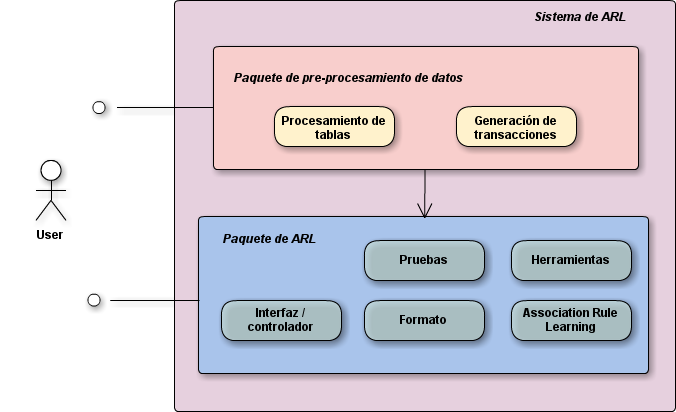
\includegraphics[width=0.9\textwidth]{imagenes/arq_sistema.png}
\end{center}
\vspace*{-5mm}
\caption{Diagrama de la arquitectura del sistema, con sus paquetes y módulos principales.}
\label{fig:arq_sistema}
\end{figure}

A continuación se detallan sus paquetes, módulos, e interfaces y explica sus funciones.

\subsection{Paquete de Association Rule Learning (ARL)}

El paquete de \textit{Association Rule Learning (ARL)} es el encargado de realizar el aprendizaje mediante reglas de asociación en sí; vale decir, de recibir un conjunto de datos con transacciones y de retornar reglas de asociación generadas a partir de aquel conjunto.

En las siguientes secciones se espacifican los formatos de entrada y salida de este paquete junto con una descripción de los módulos que lo componen.

\subsubsection{Módulo de interfaz de usuario/controlador}

El módulo de interfaz de usuario y controlador es el encargado de recibir directamente del usuario los parámetros de entrada correspondientes. Este módulo contiene métodos, clases y funciones que reciben los parámetros del usuario, abren y leen los archivos de entrada adecuados, los procesan de acuerdo al formato especificado, y hacen entrega de los datos al módulo principal de ARL.

Este módulo, es el encargado, además de recibir las reglas de asociación, entregarlas al módulo de formato para luego retornarlas al usuario en un archivo correspondiente.

\subsubsection{Módulo de formato}

Es el módulo encargado de analizar los archivos de entrada leídos por el módulo de interfaz de usuario, extraer la información pertinente de ellos según el formato especificado, y retornar los datos en una estructura adecuada para luego ser procesados por el módulo principal de ARL. A su vez, este módulo realiza, además la labor inversa; vale decir, recibe las reglas de asociación en una estructura de datos estándar para luego entregarlas al módulo de interfaz en el formato requerido por el usuario.

Hasta el momento los formatos soportados son valores separados por coma, o \textit{comma separated values (CSV)} para archivos de entrada, y CSV o tabla en formato \LaTeX\ para archivos de salida.

\subsubsection{Módulo principal de ARL}

El módulo principal de ARL es el encargado de llevar a cabo el algoritmo de aprendizaje mediante reglas de asociación en sí. En su parte lógica, consta de dos sub-módulos principales. El primero es es sub-módulo encargado de extraer los conjuntos de ítemes frecuentes; vale decir, aquellos que cumplen con el requerimiento de soporte mínimo. Y el segundo es el sub-módulo de generación de reglas, que es el encargado de recibir los conjuntos de ítemes frecuentes y generar, a partir de ellos, las reglas de asociación que cumplen con el requerimiento de confianza mínima indicado.

\subsubsection{Módulo de testeo de ARL}

Se encuentra dentro de este paquete, además, un módulo de testeo de los algoritmos de ARL sobre datos de prueba de pequeña envergadura; con el fin de realizar chequeos periódicos del funcionamiento correcto de estos algoritmos en la medida que se realizan cambios, mejoras o refactorizaciones sobre su código fuente.

\subsubsection{Módulo de herramientas}

Finalmente, se encuentra el módulo de herramientas generales, que consta de una serie de funciones de uso frecuente por parte de otros módulos del paquete; tales como operaciones sobre listas anidadas, búsqueda de llaves sobre diccionarios específicos, entre otros.

\subsection{Paquete de procesamiento de datos}

Debido a que, en la mayoría de las ocasiones los datos sobre los cuales se desea aplicar los algoritmos de reglas de asociación no se encuentran desde un comienzo en los formatos o estructuras necesarias, se procedió a implementar un paquete de pre-procesamiento. Este contiene una serie de scripts y métodos cuya función principal es extraer los datos desde sus fuentes originales, opcionalmente inferir aquella información que sea relevante, y guardarla en archivos cuyo formato sea comprensible para el paquete de aprendizaje de reglas de asociación.

En su implementación actual, este paquete se encuentra enfocado, en su mayor parte, para trabajar sobre datos extraídos a partir del Sloan Digital Sky Survey (SDSS).

A continuación se enumeran algunos de sus componentes más importantes.

\subsubsection{Queries SQL}

Una colección de queries relevantes para ejecutar en las bases de datos de SDSS y extraer los datos sobre los cuales obtener las reglas de asociación.

\subsubsection{Módulo de procesamiento de tablas}

Contiene una serie de scripts cuyo fin es recibir un archivo de tabla de base de datos en formato CSV y procesar los datos que contiene; por ejemplo, eliminando ciertas filas, añadiendo columnas calculadas a partir de las ya existentes, entre otros. Los resultados son guardados en un nuevo archivo de tabla en formato CSV.

\subsubsection{Módulo de generación de transacciones}

Este módulo contiene scripts cuya función es recibir un archivo de tabla de base de datos en formato CSV, y a partir de él generar un archivo CSV que contenga una transacción por cada fila; cada una de estas con una lista de ítemes en formato adecuado para ser recibido por el paquete de ARL.

\section{Diseño de clases}

En la Figura \ref{fig:arl_diag_clases} se observa un diagrama con las clases más importantes dentro del paquete de Association Rule Learning y sus relaciones.

\begin{figure}[h!]
\begin{center}
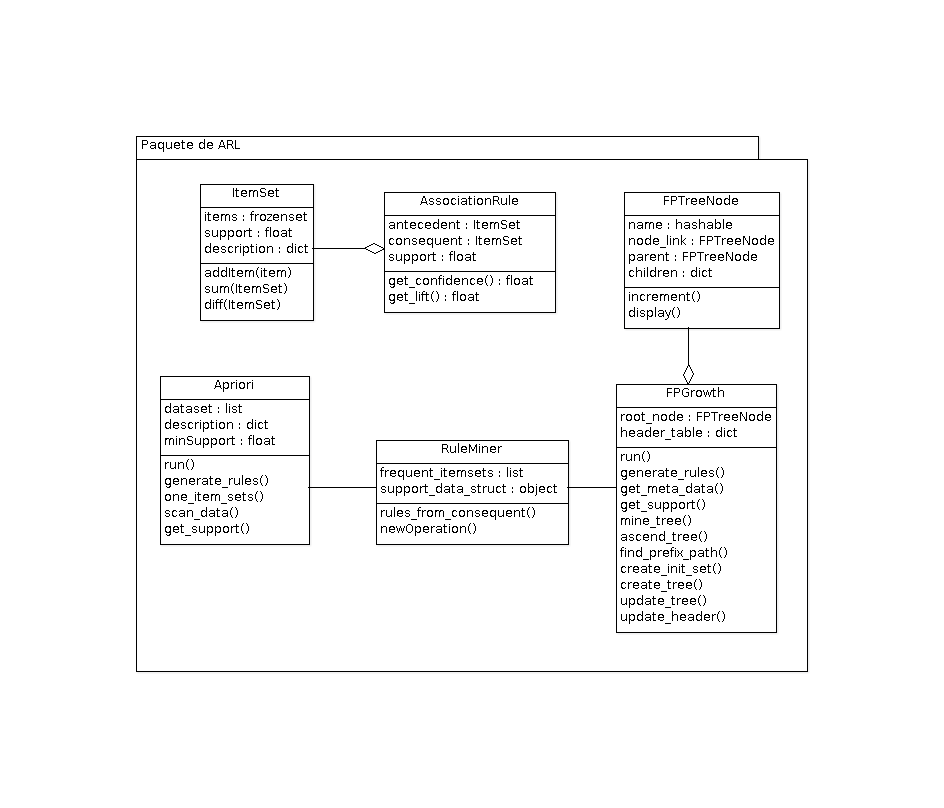
\includegraphics[width=0.9\textwidth]{imagenes/arl_diag_clases.png}
\end{center}
\vspace*{-5mm}
\caption{Diagrama de clases más importantes del paquete de ARL.}
\label{fig:arl_diag_clases}
\end{figure}

A continuación se detallan las clases de objetos más importantes del sistema.

\subsection{Clase \textit{ItemSet}}

La clase \textit{ItemSet} es la encargada de mantener información sobre un conjunto de ítemes y abstraer su estructura de datos subyacente. Cada instancia de esta clase corresponde a un conjunto de ítemes distinto, y contiene campos que guardan la información más reciente sobre su soporte (calculado sobre un cierto conjunto de transacciones) y punteros a meta-datos con información adicional sobre los ítemes en sí. Su interfaz asegura que se pueda realizar de forma adecuada, visto desde un punto de vista matemáticamente abstracto, las operaciones más comúnes de conjuntos de elementos; como comprobar pertenencia, sumar de conjuntos, diferencia entre conjuntos, entre otros.

\subsection{Clase \textit{AssociationRule}}

La clase \textit{AssociationRule} es la que define la estructura y comportamiento de las reglas de asociación. Cada instancia de esta clase corresponde a una regla de asociación en particular, extraída a partir de un cierto conjunto de datos. Cada regla de asociación consta de dos objetos de la clase \textit{ItemSet}; uno para el antecedente y otro para el consecuente de la regla. Además contiene un campo que codifica su soporte, junto con métodos para calcular sus medidas de relevancia, tales como su confianza y lift.

\subsection{Clase \textit{FrequentItemSetMiner}}

La clase \textit{FrequentItemSetMiner} es la encargada de abstraer y guardar información sobre el proceso de extraer a partir de las transacciones aquellos conjuntos de ítemes que cumplan con un requisito de soporte mínimo dado. Cada instancia de esta clase corresponde a un proceso de estracción distinto, conteniendo campos y estructuras de datos para los algoritmos involucrados, su estado actual y su resultado.

En su implementación actual, esta clase es heredada por dos sub-clases. Una correspondiente al algoritmo \textit{Apriori}, y otra al algoritmo \textit{FP-Growth}. Cada una contiene su propia implementación de los métodos principales, definidos en su clase padre, junto con sus propias funciones auxiliares y estructuras de datos correspondientes.

\subsection{Clase \textit{RuleMiner}}

La clase \textit{RuleMiner} es la que abstrae el proceso de extraer reglas de asociación a partir de conjuntos frecuentes de ítemes. Cada instancia de esta clase corresponde a un proceso de extracción distinto; básicamente el mismo en todo los casos salvo en ciertos detalles, como algunas funciones auxiliares y referencias a estructuras de datos, dependiendo de si los conjuntos fueron extraídos mediante \textit{Apriori} o \textit{FP-Growth}.

\section{Detalles de implementación}

La implementación del sistema se llevó a cabo en el lenguaje de programación Python\cite{python.org}. Se realizó una implementación propia de los algoritmos antes descritos, con algunas adaptaciones para su funcionamiento correcto en el contexto de este proyecto; y se hizo uso de paquetes externos con el fin de hacer más simple el manejo de archivos CSV y la implementación de la interfaz por línea de comando.

\subsection{Extracción de conjuntos de ítemes frecuentes}

Para la extracción de conjuntos de ítemes frecuentes se procedió a realizar la implementación de los algoritmos \textit{Apriori} y \textit{FP-Growth}. Ambos algoritmos reciben las transacciones en una misma estructura de datos y retornan los conjuntos frecuentes también en una misma estructura en ambos casos. Pero cada una de estas clases posee sus propios métodos, definidos por los algoritmos en general.

En general, para ambos algoritmos la estructura de datos más utilizada para la implementación subyacente en los objetos correspondientes a conjuntos frecuentes, candidatos, antecedentes y consecuentes por igual, fue la de \textit{frozensets}. Esta clase de objetos, además de permitir las operaciones matemáticas de conjuntos clásicas, tales como sumas y diferencias de conjuntos, permite que los objetos sean hasheables; y, por lo tanto, utilizar los conjuntos como llaves de diccionario en forma de tablas de hash, y de esta forma, por ejemplo, indexar por conjunto distintas estructuras de datos auxiliares.

\subsection{Extracción de reglas de asociación}

La extracción de reglas de asociación a partir de conjuntos frecuentes se llevó a cabo mediante una implementación del algoritmo \textit{Apriori} de generación de reglas. El sistema retorna al usuario reglas de asociación que cumplan con las medidas mínimas de soporte y confianza que él requiera. Estas serán mostradas en orden decreciente de soporte, confianza o \textit{lift}, según se requiera. Además, el sistema permite al usuario mostrar sólamente aquellas reglas en las que esté presente un cierto ítem en el antecedente o en el consecuente de ellas.

\subsubsection{Entrada y salida}

El paquete de \textit{Association Rule Learning (ARL)} recibe como entrada un archivo de tabla en formato de valores separados por coma o \textit{comma separated values (CSV)}. Este archivo debe tener el siguiente formato en cada una de sus filas

\begin{lstlisting}[basicstyle=\ttfamily]
<TID>,"<ItemList>"
\end{lstlisting}

donde \textit{<TID>} es el identificador de la presente transacción, e \textit{<ItemList>} es una lista de identificadores únicos de los ítemes presentes en la transacción separados por comas. Tal como se indica, esta lista debe ir rodeada por comillas dobles en el archivo de entrada. A continuación se muestra un ejemplo de archivo de entrada válido.

\begin{lstlisting}[basicstyle=\ttfamily]
000001,"15,2,44"
000002,"5,4,23,67,43,234"
000003,"66,3,53,23"
\end{lstlisting}

Adicionalmente, se puede especificar para cada transacción un tipo o clase a la que pertenece, o de la cual se origina, con el fin de realizar estadísticas pertinentes con las reglas generadas. De ser así, el archivo de entrada debe tener el siguiente formato en cada una de sus filas,

\begin{lstlisting}[basicstyle=\ttfamily]
<TID>,<Class>,"<ItemList>"
\end{lstlisting}

donde, en esta ocasión, se añade en la segunda posición el campo \textit{<Class>}, que consiste en una secuencia de caracteres válidos que identifique de manera unívoca la clase a la cual la transacción pertenece. A continuación un ejemplo de entrada válida en este formato.

\begin{lstlisting}[basicstyle=\ttfamily]
000001,MORNING,"15,2,44"
000002,MORNING,"5,4,23,67,43,234"
000003,NIGHT,"66,3,53,23"
\end{lstlisting}

Esta lista es leída y procesada dentro del paquete de ARL y luego entregada en una estructura de datos correspondiente al algoritmo indicado, que obtendrá las reglas de asociación presentes en el conjunto de transacciones. Estas reglas, por defecto, serán retornadas en un archivo de texto en formato CSV con la siguiente estructura en cada una de sus líneas.

\begin{lstlisting}[basicstyle=\ttfamily]
<N>,"<Antecedent>","<Consequent>",<Support>,<Confidence>,<Lift>
\end{lstlisting}

Donde \textit{N} es un número identificador de la regla de asociación, \textit{<Antecedent>} es una lista de ítemes separados por coma correspondientes al antecedente de la regla, \textit{<Consequent>} es una lista de ítemes separados por coma correspondientes al consecuente de la regla, \textit{<Support>} es un valor de punto flotante entre 0 y 1 correspondiente al soporte de la regla, \textit{<Confidence>} es un valor de punto flotante entre 0 y 1 correspondiente a la confianza de la regla, y \textit{<Lift>} es un valor de punto flotante entre 0 y 1 correspondiente al lift de la regla. A continuación un ejemplo de este formato de archivo de salida.

\begin{lstlisting}[basicstyle=\ttfamily]
1,"15,33","2,89,91",0.21,0.85,2.31
2,"12,33,44","5,23,31",0.23,0.81,3.3
\end{lstlisting}

Si, además, en los datos de entrada se especificó una clase para cada transacción, entonces el archivo de salida tendrá el siguiente formato

\begin{lstlisting}[basicstyle=\ttfamily]
<N>,"<Antecedent>","<Consequent>",<Support>,<Confidence>,
 <Lift>,"<ClassCount>"
\end{lstlisting}

en donde \textit{<ClassCount>} es una lista de valores separados por comas con el siguiente formato

\begin{lstlisting}[basicstyle=\ttfamily]
<Class01>:<Count01>,<Class02>:<Count02>,...
\end{lstlisting}

donde \textit{<Class01>} es el identificador de la primera clase, \textit{<Count01>} es un número entero que indica cuántas de las transacciones que satisfacen la regla actual pertenecen a esta primera clase, y así sucesivamente con todas las clases posibles. A continuación un ejemplo de archivo de salida con el formato recién descrito.

\begin{lstlisting}[basicstyle=\ttfamily]
1,"15,33","2,89,91",0.21,0.85,2.31,"MORNING:210,NIGHT:15"
2,"12,33,44","5,23,31",0.23,0.81,3.3,"MORNING:20,NIGHT:91"
\end{lstlisting}


\section{Interfaz de usuario}

La interfaz del usuario con el paquete principal de ARL y con los scripts del paquete de pre-procesamiento de datos, se realiza mediante un terminal o línea de comandos. Los parámetros, con los cuales se invoca cada uno de estos, siguen la sintaxis estándar \textit{de facto} de la mayoría de los sistemas tipo UNIX. En la implementación de estas interfaces se priorizó la claridad de las instrucciones por sobre lo conciso de estas, y se favorece la escritura de resultados a archivo; haciendo uso de la salida estándar solo en casos de errores y avisos del funcionamiento del sistema.

Cada uno de los archivos de entrada o interfaz de los módulos puede ser invocado con el parámetro \textit{\'-h\'} y se desplegará un texto de ayuda con los parámetros disponibles y sus funcionalidades.

Por ejemplo, el archivo de entrada del paquete de ARL, llamado \textit{spelar.py}, tiene la siguiente sintaxis de invocación:

\begin{lstlisting}[basicstyle=\ttfamily]
spelar.py [-h] [-d DESCRIPTIONS] [-l LATEX | -c CSV] (-ap | -fp)
 [-m MAX] [--by_supp] [--by_conf] [--by_lift] [--in_ant ITEM] 
 [--in_con ITEM] in_file min_supp min_conf
\end{lstlisting}\footnote{Parámetros rodeados por corchetes son opcionales. La barra vertical indica parámetros mutuamente excluyentes entre sí.}

Donde las opciones son:

\begin{itemize}
\item \texttt{-h}: Desplegar texto de ayuda.
\item \texttt{-d}: Permite especificar la ubicación de un archivo en formato CSV (\texttt{DESCRIPTIONS}) que contenga una descripción para cada identificador de ítem, para mostrar en las reglas resultantes y así ayudar a hacer más clara su semántica al usuario.
Un ejemplo de archivo de descripciones es el siguiente:
\begin{lstlisting}[basicstyle=\ttfamily]
id,description
1857,AlIII_1857
8500,CaII_8500
8544,CaII_8544
8665,CaII_8665
\end{lstlisting}
\item \texttt{-l}: Permite especificar la ubicación de un archivo (\texttt{LATEX}) en el cual escribir en formato LaTeX las reglas extraídas.
\item \texttt{-c}: Permite especificar la ubicación de un archivo (\texttt{CSV}) en el cual escribir en formato CSV las reglas extraídas.
\item \texttt{-ap}: Utilizar algoritmo Apriori para generar conjuntos frecuentes.
\item \texttt{-fp}: Utilizar algoritmo FP-Growth para generar conjuntos frecuentes.
\item \texttt{-m}: Permite especificar un número máximo \texttt{MAX} de reglas a retornar.
\item \texttt{--by\_supp}: Desplegar reglas ordenadas por soporte.
\item \texttt{--by\_conf}: Desplegar reglas ordenadas por confianza.
\item \texttt{--by\_lift}: Desplegar reglas ordenadas por lift.
\item \texttt{--in\_ant}: Mostrar sólo las reglas que posean el ítem \texttt{ITEM} en su antecedente.
\item \texttt{--in\_con}: Mostrar sólo las reglas que posean el ítem \texttt{ITEM} en su consecuente.
\item \texttt{in\_file}: Archivo de entrada en formato CSV con las transacciones.
\item \texttt{min\_supp}: Soporte mínimo de las reglas a extraer. Valor de punto flotante entre 0 y 1.
\item \texttt{min\_conf}: Confianza mínima de las reglas a extraer. Valor de punto flotante entre 0 y 1.
\end{itemize}
\chapter{Validación de la Solución}

% Demostración de cómo la solución resuelve el problema
% Dependiendo de la naturaleza del problema / solución:
% - Uso de la aplicación desarrollada en un contexto real reportando los resultados
% - Simulación de uso con un caso representativo
% - Encuesta a usuarios finales
% Dependiendo de la longitud, la validación puede ser una sección al final del capítulo de solución o un capítulo independiente

\section{Antecedentes de datos de prueba}

Explicar datos de sloan.

\section{Pre-procesamiento de datos}

Filtrado, de objetos, de líneas. Gráficos.

\section{Resultados}
\begin{conclusion}

% Breve resumen del trabajo realizado
% Recuento de objetivos alcanzados y no alcanzados
% Análisis crítico de por qué los resultados fueron los reportados
% Reflexión acerca de la relevancia / impacto del trabajo realizado
% Lecciones aprendidas
% Posibles trabajos futuros que podrían hacerse a partir de la memoria para mejorar aún más la solución



\end{conclusion}

\nocite{*}
\bibliographystyle{plain}
\bibliography{report}
\end{document}
